\documentclass[a4paper]{article}

\usepackage{polski}
\usepackage[utf8]{inputenc}

\usepackage[export]{adjustbox}
\usepackage{scrextend}
\usepackage{amsfonts}
\usepackage{amsmath}
\usepackage{svg}

\usepackage{geometry}
\geometry{a4paper, left=15mm, top=30mm, right=15mm, bottom=20mm}

\usepackage{gensymb}
\usepackage{graphicx} 
\usepackage{isotope}
\usepackage{array}
\usepackage{float}
\usepackage{titlesec}
\usepackage{fancyhdr}
\usepackage{multirow}

\usepackage{hyperref}
\usepackage{sectsty}
\usepackage{enumitem}
\usepackage{listings}
\usepackage[labelformat=simple]{subcaption}
\usepackage{xcolor,colortbl}
\usepackage{animate}

\sectionfont{\normalfont\huge\sectionrule{0pt}{0pt}{-6pt}{1pt}}
\subsectionfont{\normalfont\LARGE}

\pagestyle{fancy}
\fancyhf{}
\fancyhead[LE,LO]{\Large Łukasz Kwinta}
\fancyhead[LE,RO]{\Large Laboratorium 2 - Otoczka Wypukła}
\fancyfoot[CE,CO]{\Large\thepage}

\renewcommand{\footrulewidth}{1pt}
\renewcommand{\headrulewidth}{1pt}

\definecolor{Gray}{gray}{0.85}
\definecolor{LightGray}{gray}{0.95}

\newcolumntype{a}{>{\columncolor{Gray}}c}
\newcolumntype{b}{>{\columncolor{white}}c}

\hypersetup{
    colorlinks,
    citecolor=black,
    filecolor=black,
    linkcolor=black,
    urlcolor=black
}

\title{\fontsize{30pt}{30pt}\selectfont Laboratorium 2 \\ Otoczka Wypukła}
\author{\fontsize{20pt}{20pt}\selectfont Łukasz Kwinta}
\date{}

\begin{document}
\maketitle
\Large
\vspace*{\fill}
\section{Dane Techniczne}
Procesor: AMD Ryzen 7 5700U\\
System operacyjny: Ubuntu 20.04 w środowisku WSL 2 na Windows 11 x64\\
Pamięć ram: 32 GB DDR4\\
\\
\\
Środowisko i język: Python 3.9 + Jupyter Notebook w środowisku Anaconda\\
Wykresy tworzyłem przy pomocy narzędzia przygotowanego przez KN Bit, 
do obliczeń numerycznych używałem biblioteki numpy.
 Dane przechowywałem w zmiennych typu float – typ danych o rozmiarze 64 bitów, 
 odpowiednik typu double w języku C.
\pagebreak
\section{Opis Realizacji Ćwiczenia}
Celem ćwiczenia była implementacja algorytmów Grahama i Jarvisa do wyznaczania
otoczki wypukłej chmury punktów oraz porównanie ich precyzji oraz wydajności.

\subsection{Generowanie chmur punktów}
Pierwszym krokiem było wygenerowanie czterech zbiorów danych, które posłużą za
pierwotne przetestowania algorytmu oraz wizualizację jego działania. Wszystkie punkty
mają współrzędne 2D, typu rzeczywistego:

\begin{itemize}
    \item [a)] zawierający $100$ losowo wygenerowanych punktów o współrzędnych z przedziału $[-100, 100]$
    \item [b)] zawierający $100$ losowo wygenerowanych punktów leżących na okręgu o środku $(0,0)$ i promieniu $R=10$
    \item [c)] zawierający 100 losowo wygenerowanych punktów leżących na bokach prostokąta o wierzchołkach $(-10, 10), (-10,-10), (10,-10), (10,10)$
    \item [d)] zawierający wierzchołki kwadratu $(0, 0), (10, 0), (10, 10), (0, 10)$ oraz punkty wygenerowane losowo w sposób następujący: 
    po $25$ punktów na dwóch bokach kwadratu leżących na osiach i po $20$ punktów na przekątnych kwadratu
\end{itemize}


\noindent Liczby pseudolosowe generowałem przy pomocy funkcji bibliotecznej z biblioteki
Pythona \verb|random.uniform(left, right)| która generuje liczby typu float (odpowiednik double z języka C) 
z przedziału domkniętego $[left, right]$.
\\\\\\
\noindent Punkty ze zbioru b) generowałem przy użyciu postaci parametrycznej okręgu postaci: 
\[
(x,y)=(R\cos(2\pi t),R\sin(2\pi t)) \qquad \text{dla} \qquad t \in [0,1]
\]
Użyłem funkcji trygonometrycznych z biblioteki numpy, a parametr $t$ był zmienną losowaną.
\\\\\\
\noindent Punkty ze zbioru c) losowałem poprzez wylosowanie najpierw jednej liczby z przedziału
$[0, L]$, gdzie $L$ to obwód prostokąta, następnie sprawdzałem na którym boku znalazła się liczba,
po czym losowałem jeden punkt na odpowiednim boku.
\\\\\\
\noindent Do losowania punktów na bokach i przekątnych kwadratu użyłem funkcji generującej punkty na prostej
przechodzącej przez zadane punkty zapożyczonej z \textit{Laboratorium 1}.

\begin{table}[H]
    \centering
    \begin{tabular}{cc}
        
        \begin{subfigure}{0.5\textwidth}
            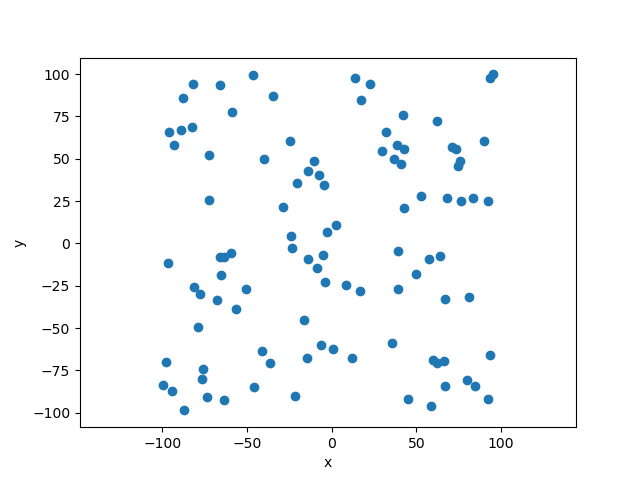
\includegraphics[width=\columnwidth]{points_a.png}
            \caption{Wizualizacja zbioru a)}
            \label{fig:points_a}
        \end{subfigure} & 
        \begin{subfigure}{0.5\textwidth}
            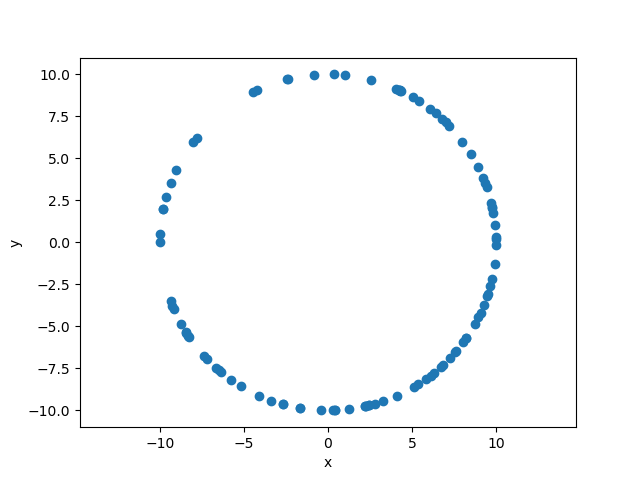
\includegraphics[width=\columnwidth]{points_b.png}
            \caption{Wizualizacja zbioru b)}
            \label{fig:points_b}
        \end{subfigure} \\

        \begin{subfigure}{0.5\textwidth}
            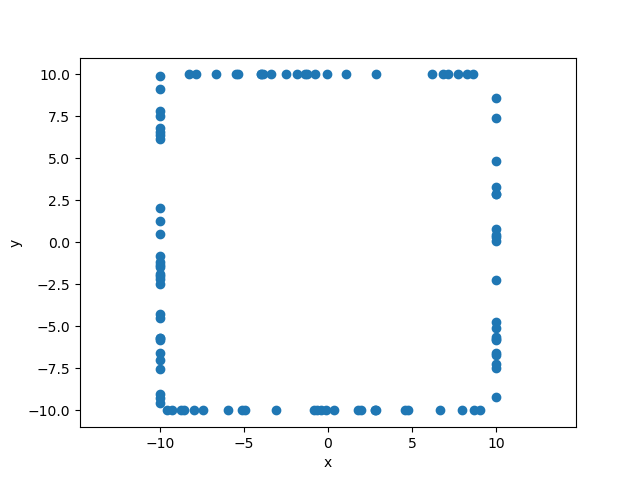
\includegraphics[width=\columnwidth]{points_c.png}
            \caption{Wizualizacja zbioru c)}
            \label{fig:points_c}
        \end{subfigure} & 
        \begin{subfigure}{0.5\textwidth}
            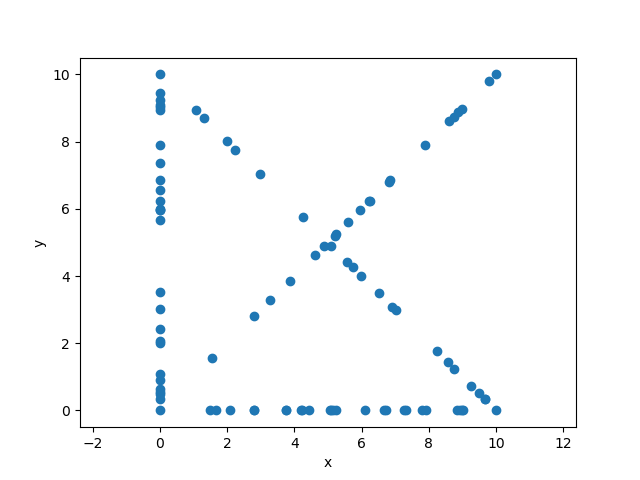
\includegraphics[width=\columnwidth]{points_d.png}
            \caption{Wizualizacja zbioru d)}
            \label{fig:points_d}
        \end{subfigure} \\
    
    \end{tabular}
    \caption{Wizualizacje zbiorów}
\end{table}

\pagebreak
\section{Algorytm Grahama}
Implementując algorytm Grahama, do sortowania punktów względem kąta użyłem wyznacznika macierzy 2x2
ze wzoru z \textit{Laboratorium 1}.
\[
    \det{(a, b, c)} = (b.x - a.x)(c.y - b.y) - (b.y - a.y)(c.x - b.x)   
\]
Aby zaoszczędzić czas na wykonywania operacji pierwiastkowania, nie obliczałem dokładnej odległości między
punktami lecz porównywałem punkty na podstawie kwadratu odległości.
\\\\\\
Do obliczeń przyjąłem dokładność zera: $\varepsilon = 10^{-32}$.\\ 
Dla tej dokładności algorytm dawał oczekiwane wyniki w
 testach przygotowanych przez KN Bit.
\\\\\\
Uproszczony schemat działania algorytmu:\\\\

\begin{enumerate}
    \item Znalezienie punktu $p_0$ o najmniejszej współrzędnej x i y
    \item Posortowanie punktów względem kąta jaki tworzą z punktem $p_0$
    \item Usunięcie współliniowych punktów z posortowanego zbioru
    \item Pamiętając 2 ostatnie punkty należące do otoczki szukamy punktów o najmniejszym kącie z nimi
\end{enumerate}

Teoretyczna złożoność tego algorytmu to:
\[O(n\log n)\]

Poniżej prezentuję wyniki działania algorytmu na poszczególnych zbiorach. W animacjach na niebiesko zaznaczam
punkty ze zbioru wejściowego, na czerwono punkty ze zbioru po usunięciu współliniowych (punkty brane pod uwagę przy wyznaczaniu otoczki),
a na zielono punkty należące do otoczki (są też one połączone linią).\\\\ 
Na rysunkach pokazujących wynik wyznaczania otoczki, na niebiesko zaznaczone są punkty wejściowe, a na zielono
punkty należące do otoczki (połączono je też linią).

\begin{figure}[H]
    \animategraphics[width=0.8\textwidth, loop, autoplay]{5}
    {graham_a_gif/graham_a-}{0}{381}
    \centering
    %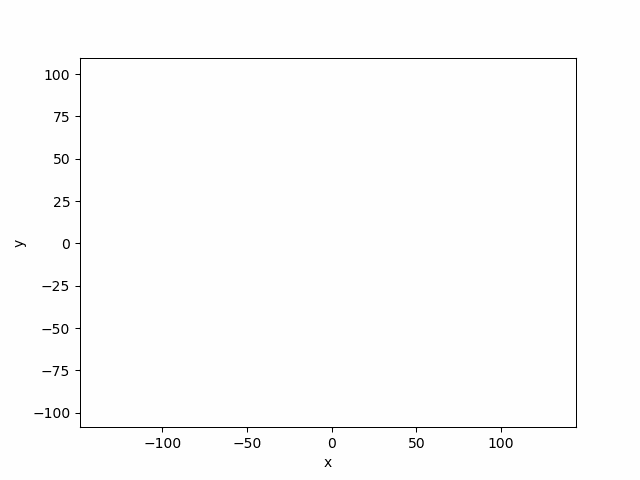
\includegraphics[width=0.8\textwidth]{graham_a_gif/graham_a-0.png}
    \caption{Animacja pokazująca działanie algorytmu Grahama na zbiorze a)}
    \label{fig:anim_graham_a}
\end{figure}

\begin{figure}[H]
    \centering
    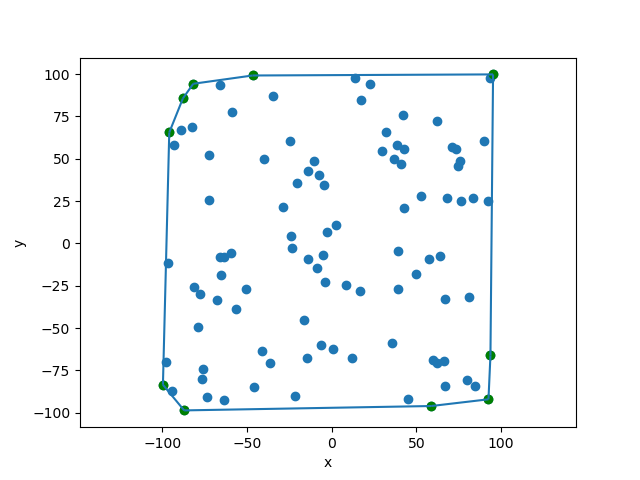
\includegraphics[width=0.8\textwidth]{graham/graham_a_png.png}
    \caption{Wynik działania algorytmu Grahama na zbiorze a)}
    \label{fig:graham_a}
\end{figure}

\begin{figure}[H]
    \animategraphics[width=0.8\textwidth, loop, autoplay]{5}
    {graham_b_gif/graham_b-}{0}{201}
    \centering
    %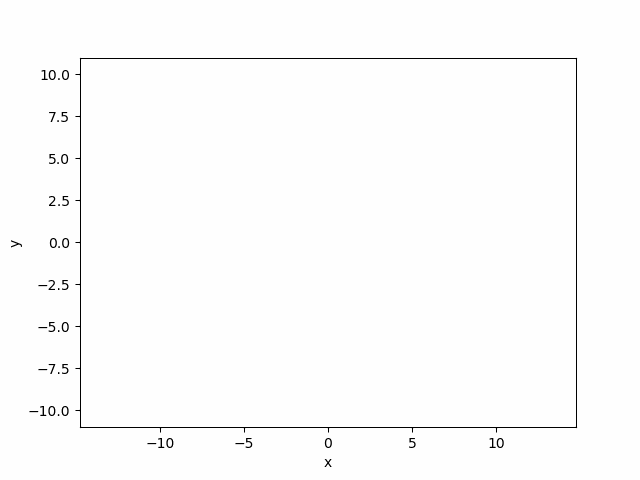
\includegraphics[width=0.8\textwidth]{graham_b_gif/graham_b-0.png}
    \caption{Animacja pokazująca działanie algorytmu Grahama na zbiorze b)}
    \label{fig:anim_graham_b}
\end{figure}

\begin{figure}[H]
    \centering
    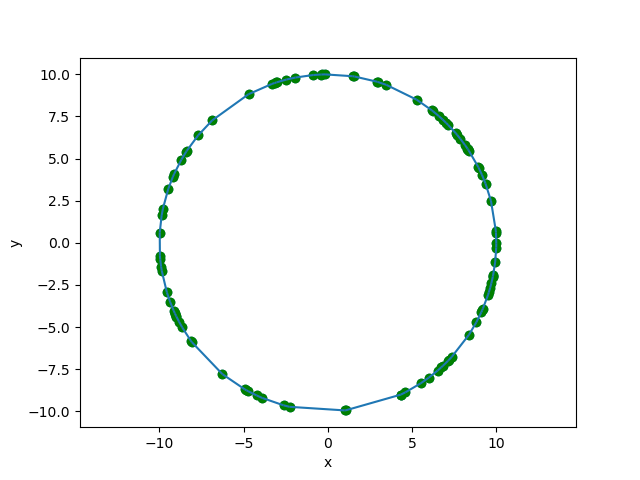
\includegraphics[width=0.8\textwidth]{graham/graham_b_png.png}
    \caption{Wynik działania algorytmu Grahama na zbiorze b)}
    \label{fig:graham_b}
\end{figure}

\begin{figure}[H]
    \animategraphics[width=0.8\textwidth, loop, autoplay]{5}
    {graham_c_gif/graham_c-}{0}{289}
    \centering
    %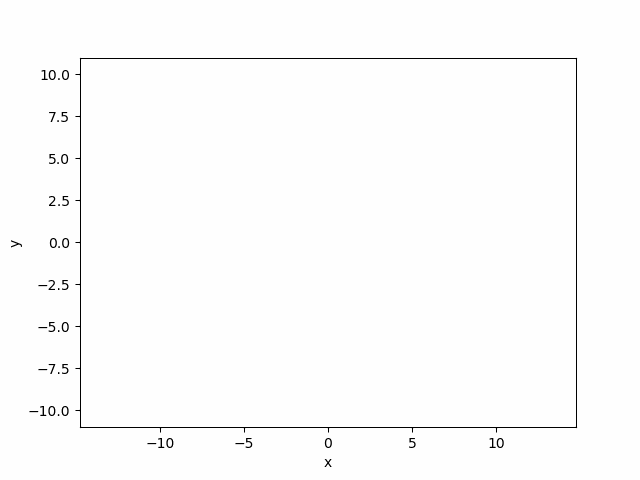
\includegraphics[width=0.8\textwidth]{graham_c_gif/graham_c-0.png}
    \caption{Animacja pokazująca działanie algorytmu Grahama na zbiorze c)}
    \label{fig:anim_graham_c}
\end{figure}

\begin{figure}[H]
    \centering
    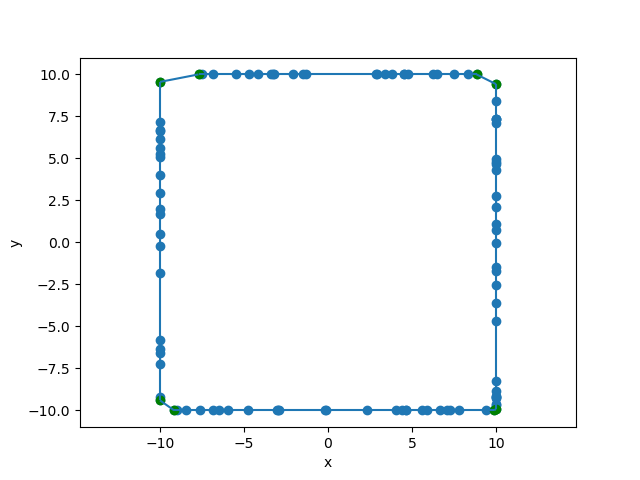
\includegraphics[width=0.8\textwidth]{graham/graham_c_png.png}
    \caption{Wynik działania algorytmu Grahama na zbiorze c)}
    \label{fig:graham_c}
\end{figure}

\begin{figure}[H]
    \animategraphics[width=0.8\textwidth, loop, autoplay]{5}
    {graham_d_gif/graham_d-}{0}{257}
    \centering
    %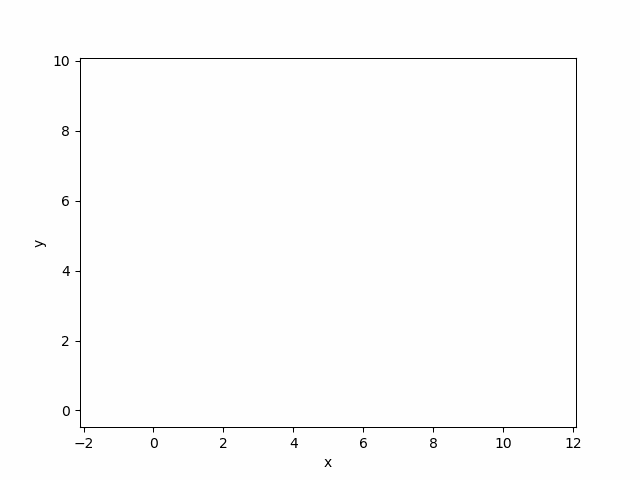
\includegraphics[width=0.8\textwidth]{graham_d_gif/graham_d-0.png}
    \caption{Animacja pokazująca działanie algorytmu Grahama na zbiorze d)}
    \label{fig:anim_graham_d}
\end{figure}

\begin{figure}[H]
    \centering
    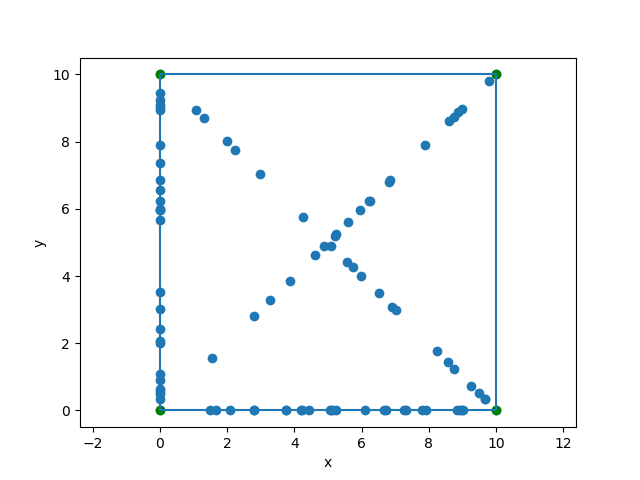
\includegraphics[width=0.8\textwidth]{graham/graham_d_png.png}
    \caption{Wynik działania algorytmu Grahama na zbiorze d)}
    \label{fig:graham_d}
\end{figure}

\section{Algorytm Jarvisa}
Wybrałem implementację algorytmu, która od razu wyznacza całą otoczkę, a nie osobno lewą i prawą stronę.\\
Do implementacji algorytmu Jarvisa, użyłem tak jak w przypadku algorytmu Grahama, użyłem wyznacznika 2x2 oraz
funkcji obliczającej kwadrat odległości pomiędzy punktami.\\
Podobnie jak wcześniej, tutaj też za dokładność zera przyjąłem wartość: $\varepsilon = 10^{-32}$.\\
Dla takiej wartości algorytm przechodził testy KN Bit.\\

Uproszczony schemat działania algorytmu:
\begin{enumerate}
    \item Wybranie punktu z najmniejszymi współrzędnymi $y$ i $x$
    \item Wybranie kandydata na następny punkt otoczki
    \item Znalezienie punktu który z ostatnimi punktami otoczki tworzy najmniejszy kąta
    \item Znaleziony punkt jest kolejnym punktem otoczki
    \item Wróć do punktu 2 o ile nie doszliśmy do pierwszego punktu otoczki
\end{enumerate}

Algorytm Jarvisa ma teoretyczną złożoność: 
\[O(n^2)\]
lecz jest on ciekawy w przypadkach gdy liczba punktów otoczki jest niewielka, wtedy
możemy ograniczyć jego złożoność przez stałą $k$ która oznacza liczbę punktów w otoczce:
\[O(kn)\]

Poniżej prezentuję animacje i wyniki działania algorytmu Jarvisa dla zadanych zbiorów danych.
Na animacjach na niebiesko oznaczono punkty wejściowe, na zielono, połączone liniami oznaczyłem punkty
tworzonej otoczki. Punkty które algorytm sprawdza w danym kroku też są oznaczone jakby to był punk otoczki
lecz można łatwo zauważyć, że są to kolejne próby znalezienia optymalnego punktu. Warto zwrócić uwagę,
że o ile w przypadku animacji dla algorytmu Grahama, zaznaczona był każdy testowany punkt, tak w tym przypadku
jako punkty przejściowe, które algorytm "testuje" zaznaczone są tylko kolejne potencjalne minima.

Na ilustracjach pokazujących wynik działania algorytmu na niebiesko zaznaczono punkty wejściowe, na zielono punkty otoczki
, dodatkowo połączone liniami.

\pagebreak
\begin{figure}[H]
    \animategraphics[width=0.8\textwidth, loop, autoplay]{5}
    {jarvis_a_gif/jarvis_a-}{0}{149}
    \centering
    %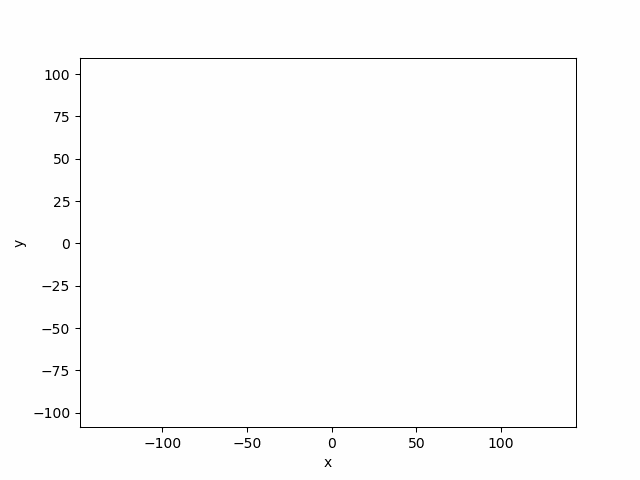
\includegraphics[width=0.8\textwidth]{jarvis_a_gif/jarvis_a-0.png}
    \caption{Animacja pokazująca działanie algorytmu Jarvisa na zbiorze a)}
    \label{fig:anim_jarvis_a}
\end{figure}

\begin{figure}[H]
    \centering
    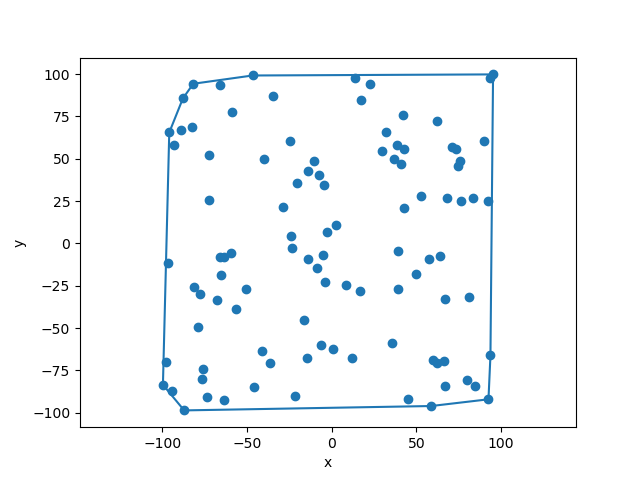
\includegraphics[width=0.8\textwidth]{jarvis/jarvis_a_png.png}
    \caption{Wynik działania algorytmu Jarvisa na zbiorze a)}
    \label{fig:jarvis_a}
\end{figure}

\begin{figure}[H]
    \animategraphics[width=0.8\textwidth, loop, autoplay]{5}
    {jarvis_b_gif/jarvis_b-}{0}{2062}
    \centering
    %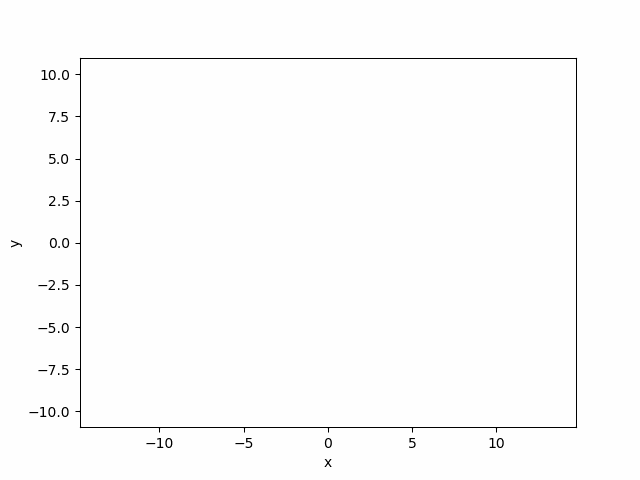
\includegraphics[width=0.8\textwidth]{jarvis_b_gif/jarvis_b-0.png}
    \caption{Animacja pokazująca działanie algorytmu Jarvisa na zbiorze b)}
    \label{fig:anim_jarvis_b}
\end{figure}

\begin{figure}[H]
    \centering
    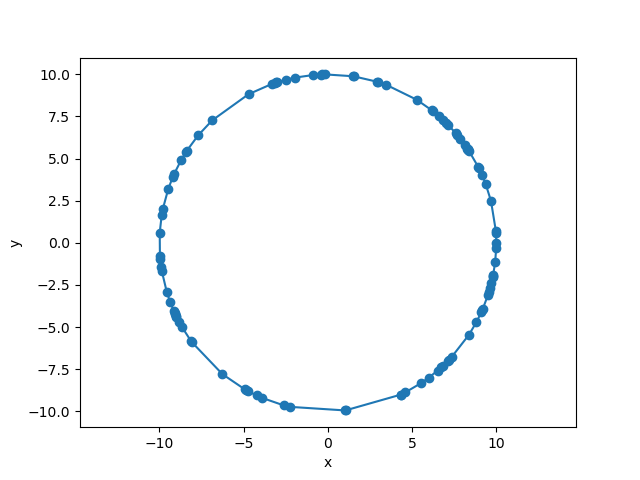
\includegraphics[width=0.8\textwidth]{jarvis/jarvis_b_png.png}
    \caption{Wynik działania algorytmu Jarvisa na zbiorze b)}
    \label{fig:jarvis_b}
\end{figure}

\begin{figure}[H]
    \animategraphics[width=0.8\textwidth, loop, autoplay]{5}
    {jarvis_c_gif/jarvis_c-}{0}{173}
    \centering
    %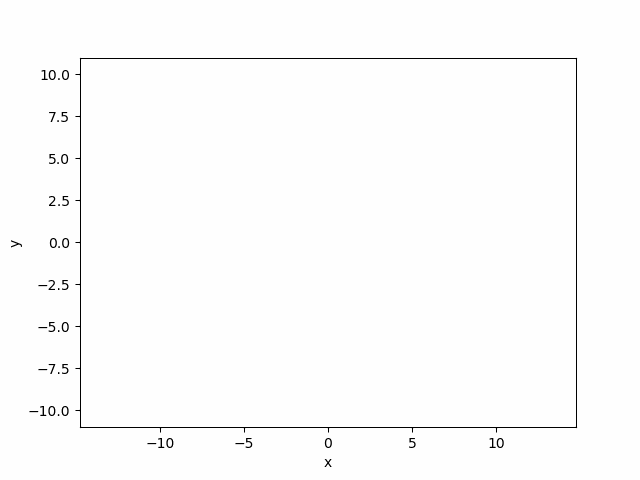
\includegraphics[width=0.8\textwidth]{jarvis_c_gif/jarvis_c-0.png}
    \caption{Animacja pokazująca działanie algorytmu Jarvisa na zbiorze c)}
    \label{fig:anim_jarvis_c}
\end{figure}

\begin{figure}[H]
    \centering
    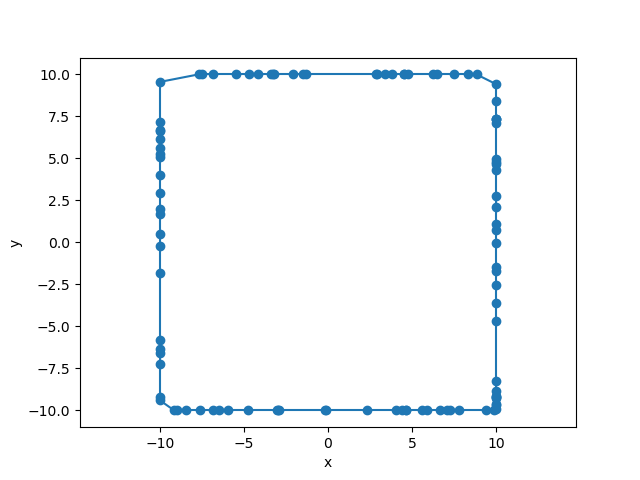
\includegraphics[width=0.8\textwidth]{jarvis/jarvis_c_png.png}
    \caption{Wynik działania algorytmu Jarvisa na zbiorze d)}
    \label{fig:jarvis_c}
\end{figure}

\begin{figure}[H]
    \animategraphics[width=0.8\textwidth, loop, autoplay]{5}
    {jarvis_d_gif/jarvis_d-}{0}{77}
    \centering
    %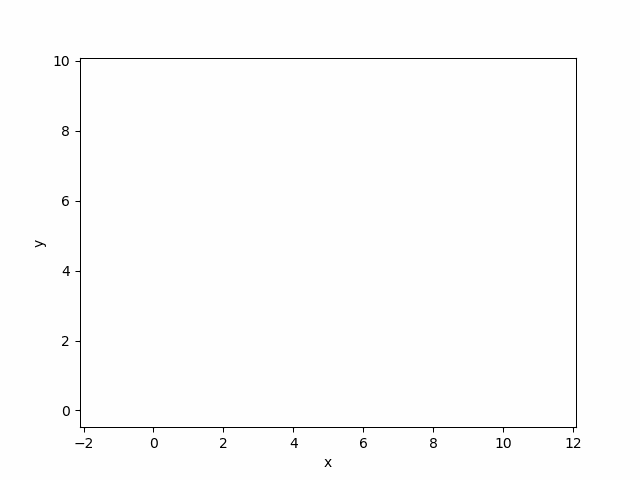
\includegraphics[width=0.8\textwidth]{jarvis_d_gif/jarvis_d-0.png}
    \caption{Animacja pokazująca działanie algorytmu Jarvisa na zbiorze d)}
    \label{fig:anim_jarvis_d}
\end{figure}

\begin{figure}[H]
    \centering
    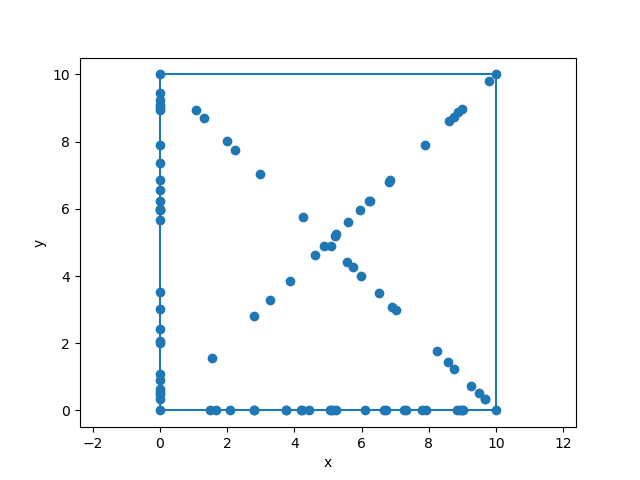
\includegraphics[width=0.8\textwidth]{jarvis/jarvis_d_png.png}
    \caption{Wynik działania algorytmu Jarvisa na zbiorze d)}
    \label{fig:jarvis_d}
\end{figure}

Już na pierwszy rzut oka widać różnicę w działaniu algorytmów. Algorytm Jarvisa wybiera punkty 
po kolei wzgledem kolejnosci ich ułożenia w tablicy, a algorytm Grahama, dzięki posortowaniu punktów,
wybiera punky względem własności.\\
Najbardziej to widać na podstawie zbioru c), gdzie algorytm Grahama na Rysunku \ref{fig:anim_graham_b}
wybiera po kolei punkty i są one od razu kwalifikowane jako punkty otoczki, a algorytm Jarvisa na 
Rysunku \ref{fig:anim_jarvis_b} skacze "losowo" po kolejnych punktach zanim trafi na punkt będący 
częścią otoczki.

\section{Modyfikacja Zbiorów}

\section{Testy Wydajnosci}
\bgroup
\def\arraystretch{2}
\begin{table}[H]
    \centering
    \begin{tabular}{|c||a|b||a|b|}
    \hline
     \multirow{2}{*}{Zbiór}        & \multicolumn{2}{c||}{Czas [s]} & \multicolumn{2}{c|}{Ilość punktów w otoczce} \\ \cline{2-5}
            & Graham & Jarvis & Graham & Jarvis\\ \hline \rowcolor{LightGray}
            Zbiór A  &  	0.000340 & 	0.001889  &	12 	    & 12    \\ \hline 
            Zbiór B  &  	0.000487 & 	0.014579  &	100     & 100   \\ \hline \rowcolor{LightGray}
            Zbiór C  &  	0.000360 & 	0.000984  &	8 	    & 8     \\ \hline
            Zbiór D  &  	0.000256 & 	0.002104  &	7 	    & 7     \\ \hline \rowcolor{LightGray}
            Zbiór A' &   	0.684662 & 	2.653454  &	27 	    & 27    \\ \hline
            Zbiór B' &   	0.006486 & 	1.214329  &	1000    & 1000  \\ \hline \rowcolor{LightGray}
            Zbiór C' &   	0.997871 & 	0.976684  &	8 	    & 8     \\ \hline
            Zbiór D' &   	6.546711 & 	2.636133  &	6 	    & 6     \\ \hline 
    \end{tabular}
    \caption{Tabela zestawiająca czas obliczania otoczki dla danych zbiorów przez oba algorytmy}
\end{table}
\egroup
\pagebreak

\section{Wnioski}
W moich testach ewidentnie szybszy okazał się algorytm Grahama, co zresztą przewiduje teoretyczna złożoność algorytmów.
Algorytm Jarvisa błyszczy gdy liczba punktów w otoczce jest niewielka, lecz w pozostałych przypadkach, przeszukiwanie całego
zbioru danych dla każdego punktu otoczki bardzo spowalnia działanie algorytmu, w tym miejscu pojawia się przewaga algorytmu 
Grahama, który sortuje punkty, dzięki czemu, później samą otoczkę może wyznaczyć liniowo.\\\\

\noindent Warto jeszcze poruszyć kwestię poprawności działania algorytmów. Oba algorytmy dały taki sam wynik dla skrajnych danych,
oba dały wyniki oczekiwane w testach przygotowanych przez KN Bit i w końcu wyniki moich testów są racjonalne, więc z całą
pewnością można stwierdzić, że algorytmy działają przewidywalnie. Na pewno nie do końca poprawnie, bo na pewno istnieją dane 
dla których przyjęta przeze mnie precyzja obliczeń nie jest odpowiednia i wynik działania programu.
\end{document}